\chapter{Method}
In this section, I will present a user-centric system for IE that attempts to tackle the issues of robustness when extracting web content. The system comes in the form of a web application, and uses a bookmarklet interface for annotation from the user.

Looking at a web information extraction system using machine learning classification techniques, the workflow of a user can be generalised into the following steps:
\begin{enumerate}
	\item The user finds a page or site that he/she would like information to be mined from.
	\item Samples of the page presented to the user for labelling. Positive examples are selected and these are fed into the machine learner to create a model.
	\item Using this model, data is extracted from similar pages, this data is then put into storage (e.g. database)
	\item Some systems repeat steps 2 and 3 iteratively until an accurate model is achieved.
	\item The user can then access the data storage for the mined information.
\end{enumerate}

The goal is to simplify this process for users of the system. In order to make it accessible, it is in the form of a web application, with a labelling interface available a bookmarklet. When the user arrives at an interesting site, he or she would then click on the available bookmarklet to begin labelling positive examples to be extracted. The bookmarklet will reduce the amount of labelling done by predicting the wanted items from the page, and this is described in Section \ref{lcas}. The result will then be sent back to the web application to be processed.
The system will then take care of updating the feeds by extracting data from the site at regular intervals. A classification model, which is described in Section \ref{classificationmodel}, is used to ensure that the extraction process is resistant to changes in the structure of the HTML page. This aims to reduce the time taken to reimplement a wrapper in case when the page is changed.

\section{System overview}
\begin{figure}[htbp]
\centering
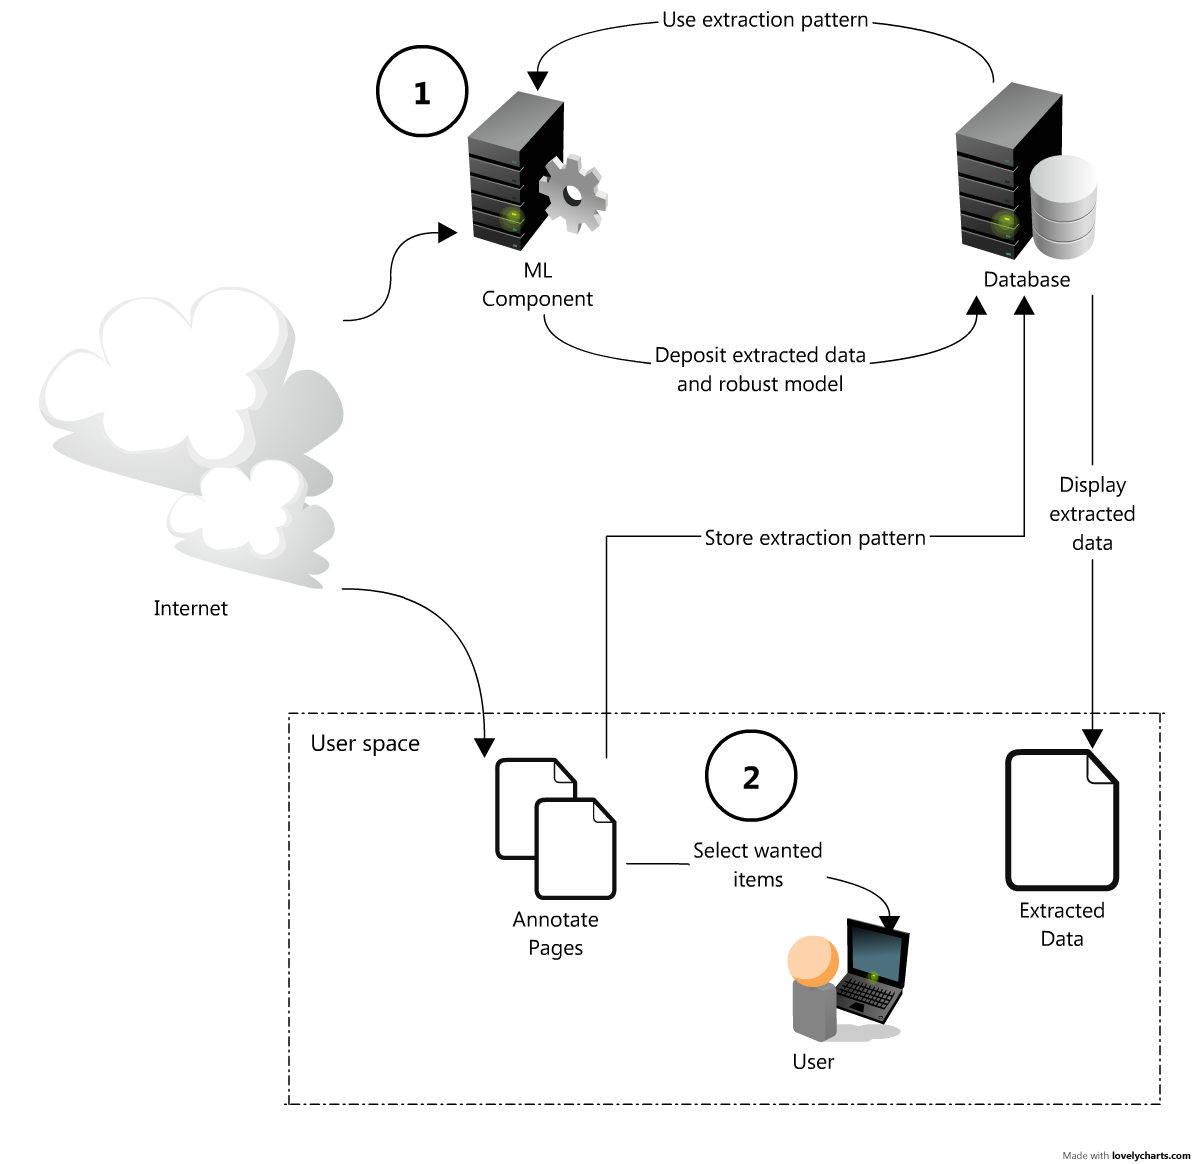
\includegraphics[scale=0.5]{parcels.png} 
\caption{Overview of the system}
\label{fig:architecture}
\end{figure}
The system comprises of 3 main components.

On the client-side, the \textbf{bookmarklet interface} allows the user to label the elements on the page he is interested in. This interface makes use of an algorithm to reduce the number of positive examples the user has to select. In this way, the labelling of documents in order to learn a classification model becomes a less tedious process.

Once the user is done with the labelling process, an XPath string is sent back to the \textbf{application server}. This component of the system provides the user interface, and at the same time has a web API to enable communication between the bookmarklet interface and the application.

The XPaths and URLs recieved will be stored on a local database, and accessed at regular intervals by the \textbf{processor}. This component will then crawl the site of interest, looking for pages similar to the one of interest to the user. From these, the machine learner will create a model of what the user has selected, which is then stored for later use. At the same time, the extacted information will then be stored on the database, and presented the next time the user accesses the web application.

\section{Bookmarklet Interface} \label{lcas}
For greater automation, the bookmarklet interface attempts to reduce the amount of labeling work the user has to do by trying to predict what the user wants to extract from the page. More specifically, as the user selects the individual HTML elements on the page using the interface, the bookmarklet attempts to generalise an XPath that captures the selected elements, and also elements on the page with similar characteristics, like class names and position within the parent tag.

\begin{figure}[htbp]
	\begin{algorithm}[H]
	\caption{\textsc{lcas($P_1,P_2$)}}
	\begin{algorithmic}[1]
		\STATE $M \leftarrow$ new array[\textsc{length}$(P_1) + 1$][\textsc{length}$(P_2) + 1$]
		\FOR{$i \leftarrow 1$ to \textsc{length}$(P_1) + 1$}
			\FOR{$j \leftarrow 1$ to \textsc{length}$(P_2) + 1$}
				\STATE $E_1 \leftarrow P_1[i]$, $E_2 \leftarrow P_2[j]$,  $E_p \leftarrow \{\}$, $M[i,j] \leftarrow E_p$
				\FOR{$a \in A$}
					\IF{$a(E_1) = a(E_2)$}
						\STATE $E_p \leftarrow E_p + \{a(E_1)\}$
						\STATE $\textsc{score}(E_p) \leftarrow \textsc{score}(E_p) + 1$			
					\ENDIF
				\ENDFOR
				\IF{$\textsc{score}(E_p) > 0$}
					\STATE $\textsc{score}(E_p) \leftarrow \textsc{score}(M[i-1][j-1])$
				\ELSE 
					\STATE $\textsc{score}(E_p) \leftarrow \textsc{Max}(\textsc{score}(M[i-1][j]),\textsc{score}(M[i][j-1]))$
					
				\ENDIF	
				\STATE $M[i,j] \leftarrow E_p$
			\ENDFOR	
		\ENDFOR
	\end{algorithmic}
	\end{algorithm}
\caption{The \textit{longest common ancestor algorithm}}
\label{fig:lcas}
\end{figure}

An important aspect which describes tags which are visually similar is its ``ancestry". Parents of selected tags with similar tag names or that have similar attributes are likely to be tags that look visually similar on the page. This also implies that the elements are probably items that that the user would also be looking for.




Given arrays of elements representing paths to 2 elements $P_1$ and $P_2$, and each element $E$ as a set of attributes $a$ in the form $a: E \to V$, where $V$ is the set of attribute values, the algorithm finds the longest common sequence (LCS) of ancestors for the selected elements. Figure \ref{fig:lcas} gives the pseudocode for the \textit{longest common ancestor algorithm} (LCAS). Modifications were made to LCS in order to find common elements within the 2 element's paths. 



This process is a bottom-up approach, since users start with a single element, and as more items are selected, the items captured by the XPath generated grows. For each element along the selected item's path, the similarties between the tag's attributes are kept, and the differences removed. This results in an extraction rule with fewer and fewer constraints as more elements are selected.

\begin{figure}[htbp]
\centering
\small
	\begin{tabular}{|l l l l l l l l|}
	\hline
	$P$ & \url{div}	&	\url{div}	&	\url{div}	&	\url{ul}	&	\url{li}	&	\url{h3}	&	\url{a} \\\hline
	id		&mainContent&	&	&	&	&	&	 \\
	index	&	4	&	1		&	1	&	3	&	\colorbox{yellow}{1}	&	1	&	1 \\
	class	&		&	content	&	newsl, pagedNewsList	&	newslTop &	&	& \\
	\hline
	\end{tabular} \\
	\begin{tabular}{|l l l l l l l l|}
	\hline
	$Q$ 	& \url{div}	&	\url{div}	&	\url{div}	&	\url{ul}	&	\url{li}	&	\url{h3}	&	\url{a} \\\hline
	id		&mainContent&	&	&	&	&	&	 \\
	index	&	4	&	1		&	1	&	3	&	\colorbox{yellow}{2}	&	1	&	1 \\
	class	&		&	content	&	newsl, pagedNewsList	&	newslTop &	&	& \\
	\hline
	\end{tabular}\\
	\textbf{After PTA:}\\
	\begin{tabular}{|l l l l l l l l|}
	\hline
	Result 	& \url{div}	&	\url{div}	&	\url{div}	&	\url{ul}	&	\url{li}	&	\url{h3}	&	\url{a} \\\hline
	id		&mainContent&	&	&	&	&	&	 \\
	index	&	4	&	1		&	1	&	3	&		&	1	&	1 \\
	class	&		&	content	&	newsl, pagedNewsList	&	newslTop &	&	& \\
	\hline
	\end{tabular}
\caption{Example of fewer constraints after each iteration}
\label{fig:lcsexample}
\end{figure}


Using alignment of the path elements, XPath rules can be generalised for elements at different levels of the DOM tree. Figure \ref{fig:lcsdiagram} is an example of a diagram generated when 2 \url{<a>} tags are compared, one at a depth of 5 from the \url{<body>} tag, and another at depth 3. The \url{<body>} tag is omitted in order to reduce the running time of the algorithm, as it is common in the paths for all visible elements on a given page. The algorithm is then able to generalise an XPath: \url{//div[@id=`main']/div//a}. This XPath will include both selected elements, as well as other anchor tags that the user may be interested in.


\begin{figure}[htbp]
\small
\centering

% The state vector is represented by a blue circle.
% "minimum size" makes sure all circles have the same size
% independently of their contents.
\tikzstyle{state}=[rectangle,
                                    thick,
                                    minimum size=1cm,
                                    draw=blue!80,
                                    fill=blue!20]
% The measurement vector is represented by an orange circle.
\tikzstyle{measurement}=[rectangle,
                                                thick,
                                                minimum size=1cm,
                                                draw=orange!80,
                                                fill=orange!25]

% The control input vector is represented by a purple circle.
\tikzstyle{input}=[rectangle,
                                    thick,
                                    minimum size=1cm,
                                    draw=red!80,
                                    fill=red!20]

% The input, state transition, and measurement matrices
% are represented by gray squares.
% They have a smaller minimal size for aesthetic reasons.
\tikzstyle{matrx}=[rectangle,
                                    thick,
                                    minimum size=1cm,
                                    draw=gray!80,
                                    fill=gray!20]

% The system and measurement noise are represented by yellow
% circles with a "noisy" uneven circumference.
% This requires the TikZ library "decorations.pathmorphing".
\tikzstyle{noise}=[circle,
                                    thick,
                                    minimum size=1.2cm,
                                    draw=yellow!85!black,
                                    fill=yellow!40,
                                    decorate,
                                    decoration={random steps,
                                                            segment length=2pt,
                                                            amplitude=2pt}]

% Everything is drawn on underlying gray rectangles with
% rounded corners.
\tikzstyle{background}=[rectangle,
                                                fill=gray!10,
                                                inner sep=0.15cm,
                                                rounded corners=2mm]

\begin{tikzpicture}[>=latex,text height=1.3ex,text depth=0.23ex]
    % "text height" and "text depth" are required to vertically
    % align the labels with and without indices.
  
  % The various elements are conveniently placed using a matrix:
  \matrix[row sep=0.3cm,column sep=0.4cm] {
    % First line: Control input
    &
        \node (u_1) [input]{\url{div[@id=`main']}}; &
        \node (u_2)   [input]{\url{div[1]}};     &
        \node (u_3) [input]{\url{ul}}; &
        \node (u_4) [input]{\url{li}}; &
        \node (u_5) [input]{\url{a}}; &
        \\
        \node (v_1)	[input]{\url{div[@id=`main']}}; &
        \node (A_1)	[input]{\url{div[@id=`main']}}; &
        \node (A_2)	[noise]{\url{div}};       &
        \node (A_3)	[matrx]{\url{NULL}};	&
        \node (A_4)	[matrx]{\url{NULL}};	&
        \node (A_5)	[matrx]{\url{NULL}};	&
        \\
        \node (v_2)	[input]{\url{div[2]}};     &
        \node (B_1)	[noise]{\url{div}};	&
        \node (B_2)	[noise]{\url{div}};     &
        \node (B_3)	[matrx]{\url{NULL}};	&
        \node (B_4)	[matrx]{\url{NULL}};	&
        \node (B_5)	[matrx]{\url{NULL}};	& 
        \\
        \node (v_3) [input]{\url{a}}; &
        \node (C_1)	[matrx]{\url{NULL}};	&
        \node (C_2)	[matrx]{\url{NULL}};	&
        \node (C_3)	[matrx]{\url{NULL}};	& 
        \node (C_4)	[matrx]{\url{NULL}};	& 
        \node (C_5)	[input]{\url{a}};	& 
        \\
        &
        \node (R_1) [measurement] {\url{div[@id=`main']}}; &
        \node (R_2)   [measurement] {\url{div}};   &
        &
        &
        \node (R_3) [measurement] {\url{a}}; &
        \\
    };
	\path[->]
		(C_5) edge[thick] (B_2)
		(B_2) edge[thick] (A_1)
		;

    \begin{pgfonlayer}{background}
        \node [background,
                    fit=(u_1) (u_5)
                    ] {};
                    
      	\node [background,
                    fit=(v_1) (v_3)
                    ] {};
        \node [background,
                    fit=(A_1) (A_5) (C_1)] {};
        \node [background,
                    fit=(R_1) (R_3),
                    label=left:Result:] {};
    \end{pgfonlayer}
\end{tikzpicture}
\caption{Table generated by the LCAS algorithm}
\label{fig:lcsdiagram}
\end{figure}

It is important to note that serialising the generalised model to its XPath form would result in loss of information. As such the model in its unserialised form is kept, and used again when another item on the page is selected. Since this process has an associative property, the order in which items are selected on the page does not matter, and the user can then select 3 items or more in order to specify the items he wants.

\section{Learning the model}\label{classificationmodel}
	Once the XPath is sent from the bookmarklet back to the server-side application and inserted into the database, the machine-learning component visits the new page inserted, and crawls within the domain for similar pages. In this context, similar pages refer to HTML documents that return results, of any number, when a query is made using any of the previously labelled XPaths. 

\begin{figure}[htbp]
\centering

\tikzstyle{action}=[rectangle,
			thick,
			minimum size=1cm,	
			draw=gray!80,
			fill=gray!20]
\tikzstyle{ml}=[rectangle,
			thick,
			minimum size=1cm,	
			draw=red!80,
			fill=red!20]
\tikzstyle{background}=[rectangle,
			fill=gray!10,
			inner sep=0.15cm,
			rounded corners=2mm]

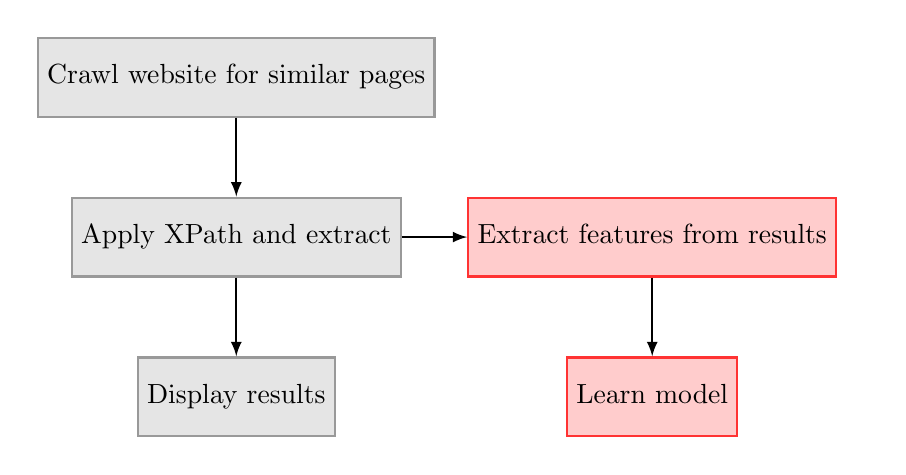
\begin{tikzpicture}[>=latex,text height=1.3ex,text depth=0.23ex]
  	\matrix[row sep=1cm,column sep=0.4cm]{
		\node (action1) [action]{Crawl website for similar pages}; 
		\\
		\node (action2) [action]{Apply XPath and extract}; &
		\node (ml1) [ml]{Extract features from results}; & 
		\\
		\node (action3) [action]{Display results}; &
		\node (ml2) [ml]{Learn model}; & 
		\\
	};
	\path[->]
	(action1) edge[thick] (action2)
	(action2) edge[thick] (action3)
	(action2) edge[thick] (ml1)
	(ml1)	edge[thick] (ml2)
	;
\end{tikzpicture}
\caption{Workflow of the machine learning component}
\label{fig:mlworkflow}
\end{figure}

	The extracted data is inserted back into the database, and then made available to the user. At the same time, features are extracted from this data in order to create a model for extraction for future use. In order to keep the model more robust and resistant to layout changes on the original site, content features are extracted in order to use less of the HTML structure for extraction. In this system, a J48 decision tree classifier is used. Positive examples of HTML elements are those returned when the XPath is applied to the given page. The following features are extracted:

	\begin{itemize}
		\item Word occurrence count (Numeric)
		\item Tag name (Discrete)
		\item Previous sibling, next sibling and parent tag name (Discrete)
		\item Number of words/tokens (Numeric)
		\item Ending with character (:,-,.) (Discrete)
		\item Header (Discrete)
	\end{itemize}
	
	For subsequent extractions, the server will first use the available XPath for extraction from the site. If the XPath rule fails to find elements for extraction, the learnt classification model is used. Figure \ref{fig:decisiontree} shows a decision tree when the process is run on a Google search result with the result entries selected for extraction.
	\begin{figure}[htbp]
\centering
% Set the overall layout of the tree
\tikzstyle{level 1}=[level distance=4cm, sibling distance=3.5cm]
\tikzstyle{level 2}=[level distance=4cm, sibling distance=2cm]

% Define styles for bags and leafs
\tikzstyle{bag} = [text width=4em, text centered]
\tikzstyle{end} = [circle, minimum width=3pt,fill, inner sep=0pt]
\tikzstyle{fork} = [circle, minimum width=3pt,fill, inner sep=0pt]
% The sloped option gives rotated edge labels. Personally
% I find sloped labels a bit difficult to read. Remove the sloped options
% to get horizontal labels. 
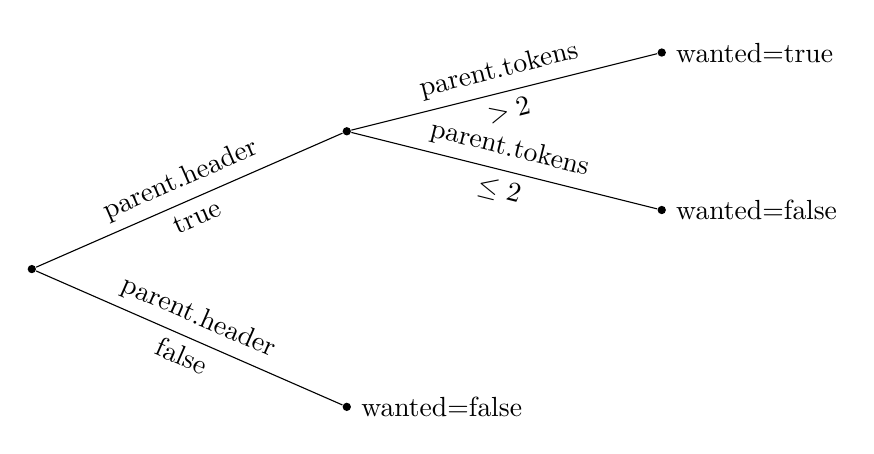
\begin{tikzpicture}[grow=right, sloped]
\node[fork] {}
    child {
        node[end, label=right:
                    {\url{wanted=false}}]{}      
	edge from parent 
            node[above] {\url{parent.header}}
            node[below]  {\url{false}}
    }
    child {
        node[fork]{}   
        child {
                node[end, label=right:
                    {\url{wanted=false}}] {}
                edge from parent
                node[above] {\url{parent.tokens}}
                node[below]  {$\leq 2$}
            }
            child {
                node[end, label=right:
                    {\url{wanted=true}}] {}
                edge from parent
                node[above] {\url{parent.tokens}}
                node[below]  {$>2$}
            }
        edge from parent         
            node[above] {\url{parent.header}}
            node[below]  {\url{true}}
    };
\end{tikzpicture}
\caption{Decision tree generated when search entries on Google are selected.}
\label{fig:decisiontree}
\end{figure}
	
	There are still some issues with the methods describe above. The items extracted from the page are still at the HTML element level. Extraction of smaller units of data which require some Natural Language Processing have not been implemented. Also, the data extracted may not be displayed in the same order as it was displayed on the original site.
